\documentclass{article}
\usepackage[table]{xcolor}
\usepackage{array}

\newcolumntype{P}[1]{>{\raggedright\vrule height4ex width 0pt}p{#1}<{\vrule depth 2.5ex width 0pt}}


\usepackage{cite}
\usepackage[unicode,pdftex]{hyperref}
\usepackage{enumerate}
\usepackage{setspace}
\usepackage{pslatex} 
\usepackage{fancyhdr}
\usepackage{float}
\usepackage{amsmath}
\usepackage{titling}
\usepackage{indentfirst}
\usepackage{graphicx}
\usepackage{wrapfig}
\usepackage{amsmath}
\usepackage{xstring}
\usepackage{tikz}
\usetikzlibrary{fit, calc}
\pagestyle{empty} 
\usepackage{array}

% \geometry{left=2.5cm, right=2.5cm, top=1.4cm, bottom=2.4cm}
\usepackage[a4paper,top=3cm,bottom=2cm,left=3cm,right=3cm,marginparwidth=1in, margin=1in]{geometry}


\title{xxxxxxxxxxxxxxxxxxxxxxxx xxxxxxxxxxxxxxxxxxxxxxxx}
\author{Wenhao You(wyou1@ualberta.ca) Leo Chang(chewei@ualberta.ca)}
\date{}

\newcommand{\reffig}[1]{Fig. \ref{#1}}
\newcommand{\refsec}[1]{Section \ref{#1}}
% \newcommand{\refeq}[1]{Eq. \ref{#1}}
\newcommand{\reftab}[1]{Table \ref{#1}}

\fancyhead{}
\lhead{\scriptsize Chenqiu Zhao}
\rhead{\scriptsize research Proposal}

\renewcommand{\headrulewidth}{0pt}
\renewcommand{\normalsize}{\fontsize{12pt}{\baselineskip}\selectfont}


\newcommand{\chronoperiode}[7]{
	\pgfmathsetmacro{\first}{(#2 - 2023)*12 + #3 - .9} % beginning of the period
	\pgfmathsetmacro{\last}{(#4 - 2023)*12 + #5 - 1.1} % end of the period
	\pgfmathsetmacro{\middle}{(\first+\last)/2} % position of the description
	
	\fill[#7] (\first,#6-1) rectangle (\last,#6) (\middle,#6-.5) node[white, font=\sf]{#1};
}


\definecolor{level1}{RGB}{200,10,20}
\definecolor{brightube}{rgb}{0.82, 0.62, 0.91}
\definecolor{fuchsia}{rgb}{1.0, 0.0, 1.0}
\definecolor{heliotrope}{rgb}{0.87, 0.45, 1.0}



\begin{document}
	\maketitle
	%\vspace{-90pt}
	
	
	
	
	
	
	\section*{Abstract}

In general, neural networks require a high-specification hardware because of their complexity. However, some researchers have a limited hardware that cannot run or train big models on their devices. In this proposal, we focus on how to implement a compression algorithm that is applied to the UNet neural network into an Android mobile device, where the algorithm is called Frequency Regularization. If the algorithm can be implemented on the mobile device, the general neural networks can also be attempted to run on limited hardware devices. As this algorithm does not reduce lots of accuracy (information?) comparing to the un-compressed neural network, it has a high possibility that we can overcome to run neural networks on the limited hardware devices and without the lost of accuracy.

Index - Compressed Neural Networks, Frequency Regularization, Limited Hardware Devices, Mobile Devices, UNet (?)


	\section*{Introduction}
	
	%\begin{wrapfigure}{l}{0.5\textwidth}
	%  \vspace{-15pt}    % 对应高度1
	%  \includegraphics[width=0.5\textwidth]{figure/fig1.pdf}\\
	%   \label{fig1}
	%  \vspace{-15pt}    % 对应高度2
	% \caption{Deep distribution Learning for Background Subtraction.}
	% \label{fig1}
	%  \vspace{-15pt}    % 对应高度3
	% \end{wrapfigure}
Neural networks have been implemented on many applications and performed a great results. However, these neural networks are mostly implemented on a high-specification hardware such as computers since there are many parameters in different neural networks. The more parameters in the neural networks, the more storages and internet transmition rates are occupied. In this research, we try to look for a method that can make the neural networks run on a limited hardware devices, such as mobile devices. Although mobile devices have more enhanced hardware nowadays, but because of its limited size, the efficacy is still not as powerful as the computers. There are several benefits of running the neural networks on limited hardware devices, specifically, mobile devices. The most important part is the privacy and the data security. Processing data on-device ensures that personal information does not need to upload or transmit to the cloud servers, which enhanced privacy. 

Running neural networks on mobile devices can also bring other advantages. If we are able to implement the neural network models directly on the mobile devices, it can reduce our dependence on the internet connection to some extent and since mobile devices play a significant role in our daily lives, it can be easily access. Moreover, for some applications which need real-time feedback, such as object recognition and image segmentation, neural networks on mobile devices can also make the process faster to improve user experience. The most important part of modern life is that we can keep the data processing and inference in our own interal system of the mobile devices rather than sending it to a remote server, which can increase the processing speed.

The new method called Frequency regularization (FR)~\cite{zhao2023frequency} is based on the frequency domain to compress the neural network. It can be divided into two steps: dynamic tail-truncation and inverse discrete cosine transform (IDCT). The main idea of this method is that some of the neural netwroks parameters may be redundant in their representation. The algorithm focus on using the frequency domain transform for network regularization to restrict information redundancy during the training process and introduce FR as shown in Fig.~\ref{idct}. Therefore, the redundant part can be removed without any side effect on the performance of the network.

\begin{wrapfigure}{l}{0.5\textwidth}
	\vspace{-15pt}    % 对应高度1
	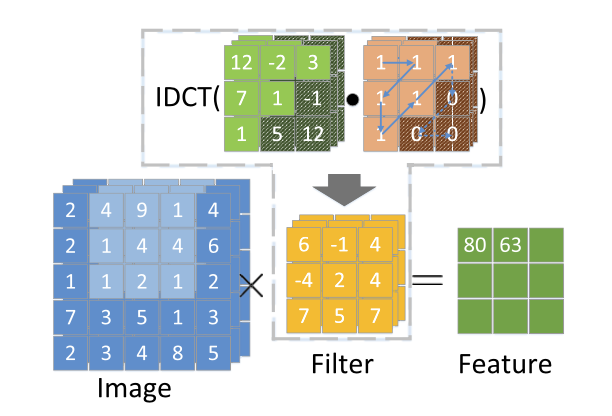
\includegraphics[width=0.5\textwidth]{figure/idct.png}\\
	\vspace{-15pt}    % 对应高度2
	\caption{Illustration of the proposed frequency regularization. The tail elements of tensors in the frequency domain are truncated first. then input into the inverse of the discrete cosine transform to reconstruct the spatial tensor for learning features~\cite{zhao2023frequency}.}
	\label{idct}
	\vspace{-15pt}    % 对应高度3
\end{wrapfigure}


In order to implement the neural networks on mobile devices, we have to think about the limitations of hardware and its characteristics. Many popular deep learning libraries, such as PyTorch and TensorFlow, are not fully complete and perfect to implement directly on the mobile devices. Thus, we need to edit some configuartions in order to optimize specifically for the mobile devices. By using this method, we can convert our standard neural network models into a lighter version that can fit the mobile devices hardware better. Moreover, beyond this idea, we can also consider improving the hardware parts such as creating special neural network processors for the mobile. In this paper, we will only explore the method in the software portion instead of the hardware.

In conclusion, this paper explores a simple, efficient, and creative method to run the large neural network on mobile devices based on Frequency regularization algorithm. Our purpose is not only to accomplish this implementation but also to make sure the performance is similar to the result running on the high-specification hardware such as computers. We hope to provide a fast and secure neural network application experience on mobile devices.


% \begin{figure}[!h]
	%     \centering
	%     \includegraphics[width=0.5\textwidth]{../imgs/distribution.pdf}
	%     \caption{Segmenting moving objects in freely moving camera.}
	%     \label{fig_intro}
	% \end{figure}

\section*{Brief Summary of Existing Work}

In this section, we cover the methods about implementing neural networks on the mobile over three sections. In Section~\ref{upgrade_hardware}, upgrading hardware on mobile devices and which part are inrtoducted. At the algorithm level, there is an algorithm called NestDNN~\cite{fang2018nestdnn} based on the dynamics or runtime resources to enable resource-aware multi-tenant on-device deep learning for mobile vision systems as shown in Section~\ref{nestdnn}. Moreover, there is an algorithm called “one-shot whole network compression”~\cite{kim2016compression} to compress convolutional neural networks (CNNs) for mobile deployment as shown in Section~\ref{oneshot}.

\subsection{Upgrade Hardware}\label{upgrade_hardware}
Hardware accelerators such as the digital signal processors offer solutions to overcome these challenges. Many manufacturers have already produced the better hardware. For example, Apple presented the Metal Performance Shaders with support of CNNs accelerated by GPU. This is a solution built on top of the Metal API and allows custom perations. Since there is a experiment~\cite{akusok2019metal} which confirmed the feasibility of Big Data analysis on modern mobile devices. Moreover, the hardwares on Android devices are upgraded by four main companies, such as Qualcomm , HiSilicon, MediaTek, and Samsung~\cite{Andrey2019Aibenchmark}, which can be used for neural networks as well.

\subsection{Algorithm NestDNN}\label{nestdnn}
NestDNN is a framework that takes the dynamics of runtime resources into account to enable resourceaware multi-tenant on-device deep learning for mobile vision systems. NestDNN enables each deep learning model to offer flexible resource-accuracy trade-offs~\cite{fang2018nestdnn}. Fig.~\ref{nestdnn_arch} illustrates the architecture of NestDNN detailedly, which is split into an offline stage and an online stage. The offline stage consists of three phases: model pruning, model recovery, and model profiling~\cite{fang2018nestdnn}. In Table~\ref{table_nestdnn}, it illustrates all the terminologies involved in NestDNN.

	\begin{figure}[htbp]
	\centering
	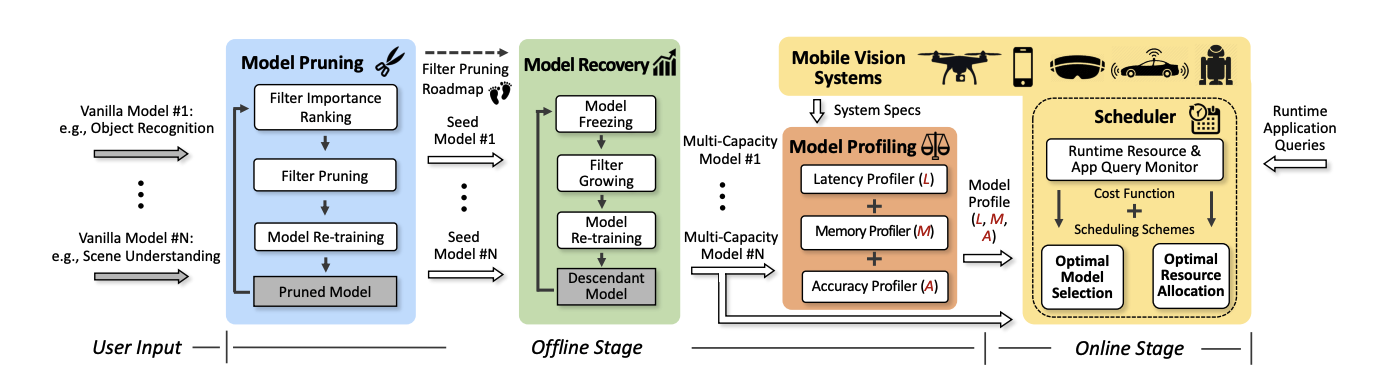
\includegraphics[width=1\linewidth]{figure/nestdnn_architecture.png}
	\caption{NestDNN architecture~\cite{fang2018nestdnn}.}
	\label{nestdnn_arch}
\end{figure}

\begin{table}
	\label{table_nestdnn}
	\centering
	\begin{tabular}{|c|>{\centering\arraybackslash}p{8cm}|}
		\hline
		\textbf{Terminology}&\textbf{Explanation}\\
		\hline
		\textbf{Vanilla Model}&Off-the-shelf deep learning model (e.g., ResNet) trained on a given dataset (e.g., ImageNet). \\
		\hline
		\textbf{Pruned Model}&Intermediate result obtained in model pruning stage.\\
		\hline
		\textbf{Seed Model}&The smallest pruned model generated in model pruning which meets the minimum accuracy goal set by the user. It is also the starting point of model recovery stage.\\
		\hline
		\textbf{Descendant Model}&A model grown upon the seed model in model recovery stage. It has a unique resource-accuracy trade-off.\\
		\hline
		\textbf{Multi-Capacity Model}&The final descendant model that has the capacities of
		all the previously generated descendant models.\\
		\hline
	\end{tabular}
	\caption{Terminologies involved in NestDNN~\cite{fang2018nestdnn}.}
\end{table}


\subsection{Algorithm One-shot Whole Network Compression}\label{oneshot}
"One-shot Whole Network Compression" is a simple way to compress CNNs to make them more suitable for fast and low-power applications on the mobile. This algorithm can be divided into three steps: rank selection, tensor decomposition, and fine-tuning. Each step can be implemented easily by using public tools such as VBMF for rank selection, Tucker decomposition for tensor decomposition, and Caffe for fine-tuning~\cite{kim2016compression}.

\section*{What you Plan To Do}
There are five sub-topics for implementing Frequency Regularization on the Android devices. The first one "Implement Frequency Regularization" have done in Basu's lab in University of Alberta (2023). The remaining topics will be finished before the lecture ends.


\begin{itemize}
	\item Implement Frequency Regularization: Implement the Frequency Regularization in order to compress the redundant information on nerual network. Make sure that the accuracy and velocity is acceptable for the nerual network.
	
	\item Configure Emulator: In this paper, we choose Android Studio as our emulator. Install it successfully on our own local machines.
	
	\item Implement PyTorch Library: Implement PyTorch Android libaray to the emulator. Collect and analyze the error information if we get.
	
	\item Adjust Dependencies: Potential errors may probably caused by Android PyTorch Library. Since the library on android lacks of improvement not as much as laptop.
	
	\item Adjust Frequency Regularization: We can also try to change something on the algorithm to let the new one fitting the Android system.
	
\end{itemize}

\section*{How You Plan to Implement Your Ideas}

In this research, we are only going to put the compressed neural network to the mobile devices and make it run on the emulator. 



\section*{Timeline}

\begin{tikzpicture}[x=9mm,y=7mm]
	% draw the grid
	\draw[help lines] (0,0) grid[step=1] (12, 4);
	% \draw (0,0) grid[xstep=2,ystep=7] (12,7);
	% put months and years under the x-axis
	\foreach[count=\a] \aa in {10,...,12} {
		\draw[gray] (4*\a-4,0) -- +(0,-7mm) node[pos=.5, below right, inner sep=1pt]{2023. $\aa$};
		\foreach[count=\m] \mm in {Week1, Week2, Week3, Week4}
		\node[font=\tiny,below,gray] at (4*\a+\m-4.5,0) {\mm};
	}
	
	% plot the data
	
	\chronoperiode{Review of Existed Work}{2018}{10}{2018}{11}{1}{level1}
	\chronoperiode{Experiments}{2018}{5}{2019}{1}{2}{cyan}
	\chronoperiode{Paper Writing}{2018}{6}{2019}{5}{3}{brightube}
	%      \chronoperiode{HLDR}{2019}{4}{2019}{11}{4}{fuchsia}
	%      \chronoperiode{test}{2018}{4}{2019}{10}{1}{olive}
	%      \chronoperiode{Incorporating spatial information}{2018}{10}{2019}{10}{2}{cyan}
\end{tikzpicture}

\section*{Short Description of 5 LABS}

In this paper, we will divide the project into five labs (milestones), which can help us to double check our progress and adjust it timely.

\begin{itemize}
	\item Deploy the Frequency Regularization algorithm with the UNet (one basic Neural Network) on the computer and adjust some parameters for the Android emulator. 
	
	\item Attempt to implement PyTorch on the emulator and summarize the error messages.
	
	\item Analyze the error messages and try to do the debug process. 
	
	\item xxxxxxxxxxxxxxxxxxxxxxxxxxxxxxxxxxxxxxxxxxxxxxxxxxxxxxx
	
	\item Test all functions and neural networks to check the effectiveness and accuracy on the emulator after importing the compressed neural network. We compare the result between the computer and mobile devices. 
	
\end{itemize}



\small
\bibliographystyle{unsrt}
% \bibliographystyle{plain}
\bibliography{ref.bib}  




\end{document}
